

\tikzset{every picture/.style={line width=0.75pt}} %set default line width to 0.75pt        

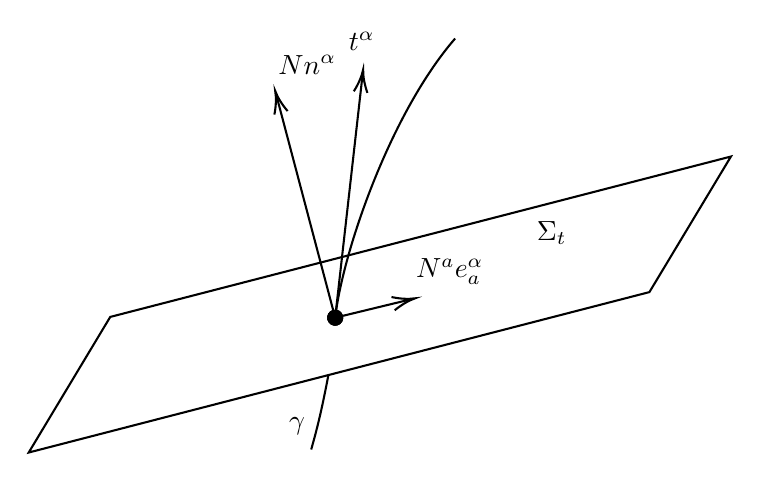
\begin{tikzpicture}[x=0.75pt,y=0.75pt,yscale=-1,xscale=1]
	%uncomment if require: \path (0,215); %set diagram left start at 0, and has height of 215
	
	%Shape: Parallelogram [id:dp07267193688534523] 
	\draw   (203.32,145.77) -- (502.37,68.49) -- (463.09,133.81) -- (164.04,211.1) -- cycle ;
	%Curve Lines [id:da020936867256896807] 
	\draw    (311.69,146.14) .. controls (315.54,113.45) and (338.66,47.14) .. (369.47,11.65) ;
	%Straight Lines [id:da48198359303560534] 
	\draw    (311.69,146.14) -- (283.31,38.8) ;
	\draw [shift={(282.8,36.87)}, rotate = 435.19] [color={rgb, 255:red, 0; green, 0; blue, 0 }  ][line width=0.75]    (10.93,-3.29) .. controls (6.95,-1.4) and (3.31,-0.3) .. (0,0) .. controls (3.31,0.3) and (6.95,1.4) .. (10.93,3.29)   ;
	\draw [shift={(311.69,146.14)}, rotate = 255.19] [color={rgb, 255:red, 0; green, 0; blue, 0 }  ][fill={rgb, 255:red, 0; green, 0; blue, 0 }  ][line width=0.75]      (0, 0) circle [x radius= 3.35, y radius= 3.35]   ;
	%Straight Lines [id:da16137864605187602] 
	\draw    (311.69,146.14) -- (324.95,28.58) ;
	\draw [shift={(325.17,26.59)}, rotate = 456.43] [color={rgb, 255:red, 0; green, 0; blue, 0 }  ][line width=0.75]    (10.93,-3.29) .. controls (6.95,-1.4) and (3.31,-0.3) .. (0,0) .. controls (3.31,0.3) and (6.95,1.4) .. (10.93,3.29)   ;
	\draw [shift={(311.69,146.14)}, rotate = 276.43] [color={rgb, 255:red, 0; green, 0; blue, 0 }  ][fill={rgb, 255:red, 0; green, 0; blue, 0 }  ][line width=0.75]      (0, 0) circle [x radius= 3.35, y radius= 3.35]   ;
	%Straight Lines [id:da6584082424480233] 
	\draw    (311.69,146.14) -- (348.27,137.27) ;
	\draw [shift={(350.21,136.8)}, rotate = 526.37] [color={rgb, 255:red, 0; green, 0; blue, 0 }  ][line width=0.75]    (10.93,-3.29) .. controls (6.95,-1.4) and (3.31,-0.3) .. (0,0) .. controls (3.31,0.3) and (6.95,1.4) .. (10.93,3.29)   ;
	\draw [shift={(311.69,146.14)}, rotate = 346.37] [color={rgb, 255:red, 0; green, 0; blue, 0 }  ][fill={rgb, 255:red, 0; green, 0; blue, 0 }  ][line width=0.75]      (0, 0) circle [x radius= 3.35, y radius= 3.35]   ;
	%Curve Lines [id:da5810666182622253] 
	\draw    (308.45,173.65) .. controls (304.95,191.9) and (303.03,199.37) .. (300.14,209.64) ;
	
	
	% Text Node
	\draw (288.04,192.8) node [anchor=north west][inner sep=0.75pt]    {$\gamma $};
	% Text Node
	\draw (316.84,6.91) node [anchor=north west][inner sep=0.75pt]    {$t^{\alpha }$};
	% Text Node
	\draw (282.86,18.12) node [anchor=north west][inner sep=0.75pt]    {$Nn^{\alpha }$};
	% Text Node
	\draw (349.23,116.12) node [anchor=north west][inner sep=0.75pt]    {$N^{a} e_{a}^{\alpha }$};
	% Text Node
	\draw (407.33,98.44) node [anchor=north west][inner sep=0.75pt]    {$\Sigma _{t}$};
	
	
\end{tikzpicture}